\documentclass[11pt]{article}
\usepackage[margin=1.1in]{geometry}
\usepackage{amsmath,amssymb,bm}
\usepackage{booktabs}
\usepackage{siunitx}
\usepackage{graphicx}
\usepackage{tikz}
\usetikzlibrary{arrows.meta,positioning}
\usepackage[colorlinks=true,linkcolor=blue,citecolor=blue,urlcolor=blue]{hyperref}

\newcommand{\ud}{\,\mathrm{d}}
\newcommand{\vect}[1]{\bm{#1}}
\newcommand{\Rhat}{\hat{\vect{R}}}
\newcommand{\That}{\hat{\vect{T}}}
\newcommand{\Nhat}{\hat{\vect{N}}}

\title{Minimum-Fuel Elliptic-to-GEO Transfer with Lunar Gravity:\\
Problem Formulation, Third-Body Incorporation, and the First Certified Result}
\author{Michael Casey}
\date{July 22, 2026}

\begin{document}
\maketitle

\begin{abstract}
We extend a certified\footnote{``Certified'' throughout means a
solver-level, \emph{first-order} certificate: full IPOPT convergence
(\texttt{Solve\_Succeeded}), post-hoc numerically re-checked collocation
defects, and endpoint/structure gates --- not a proof of global (or even
local) optimality. See \S\ref{sec:certification} for the exact basis and
\S\ref{sec:minimality} for what a stronger certificate would require.}
two-body low-thrust minimum-fuel campaign --- the
Haberkorn--Martinon--Gergaud (HMG) elliptic-orbit-to-GEO benchmark --- to
include the Moon's gravity at circular-restricted three-body (CR3BP)
fidelity --- i.e.\ the ideal circular-restricted model expressed in a
geocentric, non-rotating frame, not the traditional rotating-frame CR3BP
formulation --- while retaining the two-body campaign's winning
formulation: modified equinoctial elements (MEE) with true longitude as
the independent variable and a \emph{free} total longitude span. The Moon
enters as an Earth-centered third-body perturbation (direct plus indirect
terms) added to the Gauss variational equations as a pure acceleration.
The three-body solution is reached by lunar-gain continuation from the
certified two-body solution on the smooth energy objective, followed by an
energy$\to$fuel homotopy at full lunar mass. At the 10\,N rung the certified
result is $m_f = 1377.1545$\,kg against the \emph{same-chain} two-body
control $1377.1025$\,kg ($\varphi_0 = 0$, identical seed/mesh/continuation
path): the Moon \emph{improves} the transfer by $+52.0$\,g ($+0.004\%$) at
the baseline lunar phase, a same-chain differenced value, in agreement with
an a~priori tidal null model. The completed thrust ladder ($10 \to 0.1$\,N)
shows this fixed-phase benefit declining from $+52.0$\,g to $+31.3$\,g. This
note records the optimal control problem, the lunar incorporation, the
continuation strategy, and the certification basis.
\end{abstract}

\section{The benchmark problem}
\label{sec:benchmark}

The underlying problem is the HMG-2004 benchmark \cite{HMG2004}: transfer a
low-thrust spacecraft of initial mass $m_0 = 1500$\,kg from an inclined
elliptic orbit
\[
P^0 = 11\,625~\text{km}, \qquad e^0 = 0.75, \qquad i^0 = 7^\circ,
\qquad \text{(apogee start, } L_0 = \pi\text{)}
\]
to the geostationary orbit ($P_f = 42\,165$\,km, $e_f = 0$, $i_f = 0$),
maximizing final mass at fixed transfer time $t_f = 1.5\,t_f^{\min}(T)$,
where $t_f^{\min}(T)$ is the certified minimum time at thrust level $T$.
The benchmark constants derive from Caillau--Noailles \cite{CN2001}
($I_{sp} \simeq 1995$\,s; we use the campaign's 2000\,s convention). The
two-body campaign certified the full thrust ladder $10 \to 0.1$\,N; at the
10\,N rung considered here, $t_f = 33.3309$\,TU $= 5.290$\,d and the
certified two-body final mass is $1377.1000$\,kg.

The question posed to the three-body campaign is quantitative: \emph{how
much does lunar gravity move the certified two-body answers} --- final
mass, switch structure, and ultimately the ladder laws --- under identical
boundary conditions and time budget?

\section{The optimal control problem}

\subsection{State, control, and dynamics}

We work in modified equinoctial elements with true longitude $L$ as the
independent variable. The state and control are
\[
X = \left[\,P,\ e_x,\ e_y,\ h_x,\ h_y,\ m,\ t\,\right]^{\!\top},
\qquad
U = \left[\,\vect{\beta};\ \delta\,\right],
\quad \lVert \vect{\beta} \rVert = 1,\ \ \delta \in [0,1],
\]
where $(P, e_x, e_y, h_x, h_y)$ are the usual MEE
($h_x = \tan\tfrac{i}{2}\cos\Omega$, $h_y = \tan\tfrac{i}{2}\sin\Omega$),
$m$ is the mass, $t$ is carried as a state, $\vect{\beta}$ is the unit
thrust direction in the local RTN (radial--transverse--normal) frame, and
$\delta$ is the throttle. With canonical units $\mu_E = 1$,
$\mathrm{LU} = 42\,165$\,km (so GEO circular speed is unity), the induced
time unit is $\mathrm{TU} = \sqrt{\mathrm{LU}^3/\mu_{E,\mathrm{km}}}
\approx 13{,}714$\,s (with $\mu_{E,\mathrm{km}} = 398\,600.4418$\,km$^3$/s$^2$,
consistent with $t_f = 33.3309$\,TU $= 5.290$\,d, \S\ref{sec:benchmark});
every dimensional quantity used below --- the lunar acceleration $a_M$
built from $\mu_M$ and $D_{EM}$ (native km, s), the thrust authority
$T_{\max}/m$ and exhaust velocity $c$ (native m, s), and the time state
$t$ itself --- is converted through this single (LU, TU) pair before
entering the canonical equations. The dynamics that result are the Gauss
variational equations driven by the RTN specific force
$\vect{f} = (f_R, f_T, f_N)$, written here as ordinary \emph{time} rates
$\dot X$ --- i.e., before the $\sigma$-domain transcription applied at the
end of this subsection:
\begin{equation}
\label{eq:gauss}
\begin{aligned}
\dot P   &= \frac{2P}{Z}\sqrt{\tfrac{P}{\mu}}\; f_T, \\
\dot e_x &= \sqrt{\tfrac{P}{\mu}}\,\tfrac{1}{Z}
            \bigl( Z \sin L\, f_R + A_1 f_T - e_y (h_x \sin L - h_y \cos L) f_N \bigr), \\
\dot e_y &= \sqrt{\tfrac{P}{\mu}}\,\tfrac{1}{Z}
            \bigl( -Z \cos L\, f_R + A_2 f_T + e_x (h_x \sin L - h_y \cos L) f_N \bigr), \\
\dot h_x &= \tfrac{1}{2}\sqrt{\tfrac{P}{\mu}}\,\tfrac{X_h}{Z} \cos L\, f_N, \qquad
\dot h_y = \tfrac{1}{2}\sqrt{\tfrac{P}{\mu}}\,\tfrac{X_h}{Z} \sin L\, f_N, \\
\dot L   &= \sqrt{\tfrac{\mu}{P^3}}\,Z^2
            + \sqrt{\tfrac{P}{\mu}}\,\tfrac{1}{Z}\,(h_x \sin L - h_y \cos L)\, f_N, \\
\dot m   &= -\tfrac{T_{\max}}{c}\,\delta, \qquad \dot t = 1,
\end{aligned}
\end{equation}
with $Z = 1 + e_x\cos L + e_y \sin L$, $A_1 = e_x + (1{+}Z)\cos L$,
$A_2 = e_y + (1{+}Z)\sin L$, $X_h = 1 + h_x^2 + h_y^2$, and exhaust
velocity $c = I_{sp} g_0$. In the two-body problem the specific force is
thrust alone, $\vect{f} = (T_{\max}/m)\,\delta\vect{\beta}$.

To make $L$ the independent variable, every trajectory quantity is
transcribed on a fixed grid $\sigma \in [0,1]$ with node longitudes
$L_k = \pi + \sigma_k \Delta L$, i.e.\ $L = \pi + \sigma \Delta L$ and
$dL/d\sigma = \Delta L$. By the chain rule, the state (and the time state
$t$) are propagated in $\sigma$ as
\begin{equation}
\label{eq:sigmadomain}
\frac{dX}{d\sigma} = \Delta L\,\frac{\dot X}{\dot L},
\qquad
\frac{dt}{d\sigma} = \frac{\Delta L}{\dot L},
\end{equation}
i.e.\ every rate in \eqref{eq:gauss} --- including $\dot t = 1$ --- is
divided by $\dot L$ and scaled by $\Delta L$ before collocation. This
division is well posed only if $\dot L > 0$ throughout the transfer
(longitude increasing monotonically); that condition is enforced/checked
in the implementation and holds for this GEO-bound, non-librating
geometry.

\subsection{Free longitude span}

The total swept longitude $\Delta L$ is a single scalar \emph{decision
variable} of the problem --- the transfer's revolution count is chosen by
the optimizer, not prescribed. This is the formulation feature that carried
the two-body ladder through two thrust decades (rev counts from
$\sim$7 to $\sim$700), and preserving it was the decisive argument for
incorporating the Moon as a perturbation in this frame rather than moving
to rotating-frame Cartesian coordinates, where a fixed independent-variable
span makes it difficult in practice --- for a fixed mesh and warm start ---
for the optimizer to add or shed a revolution.

\subsection{Fixing $t_f$: two inequivalent transcriptions}

It is worth being precise about what ``fixed transfer time'' means here,
because two formulations that both \emph{fix $t_f$} are not equivalent.
The direct way is to make time (or a regularized time such as a Sundman
variable) the independent variable and fix the mesh span: the horizon of
the transcription itself is $[0, t_f]$. This is the formulation of our
CR3BP GTO campaigns, and its practical cost is a conditioning/mesh
limitation rather than a mathematical impossibility: with the
independent-variable span fixed, the trajectory's revolution count is tied
to the warm start's geometry, and it is difficult in practice for the
optimizer to add or shed a revolution without re-meshing or a fresh warm
start --- this is the ``topology wall'' those campaigns meet under thrust
continuation.

What we do here is different: the independent variable is $L$ with a
\emph{free} span $\Delta L$, physical time is demoted to a state with
$\dot t = 1$, and the time budget enters only as a terminal
\emph{constraint} $t(1) = t_f$ on that state. The same physical quantity
is fixed, but as a boundary condition rather than as the mesh horizon ---
so the optimizer retains the winding freedom while honoring the time
budget exactly. The distinction parallels the MfMax family of indirect
solvers \cite{HMG2004}: their v0 fixes both $t_f$ and the final longitude
$L_f$; their v1 frees $t_f$ (with transversality) at fixed $L_f$; our
formulation is the reciprocal of v1 --- $t_f$ fixed, $L_f$ free --- and it
is this reciprocal choice that lets one solver family sweep the thrust
ladder, where rev counts change by two orders of magnitude, without ever
re-meshing in time.

\subsection{Objective and homotopy}

The physical objective is maximum final mass, equivalently minimum fuel:
\begin{equation}
\min_{\delta(\cdot),\,\vect{\beta}(\cdot)} \int_0^{t_f} \delta \ud t ,
\qquad t(1) = t_f \ \text{pinned}.
\end{equation}
The bang-bang structure of the $L^1$ objective is reached through the
Bertrand--\'Ep\'enoy convex homotopy \cite{BE2002}
\begin{equation}
J_\varepsilon \;=\; \int_0^{t_f}
\bigl[\, \delta \;-\; \varepsilon\, \delta(1-\delta) \,\bigr] \ud t,
\qquad \varepsilon: 1 \to 0,
\end{equation}
for $\varepsilon \in [0,1]$. At $\varepsilon = 1$ the integrand collapses
to $\delta - \delta(1-\delta) = \delta^2$, so $J_1 = \int_0^{t_f}
\delta^2\,\ud t$ --- a \emph{quadratic throttle (energy) surrogate}, which
we refer to below by the shorthand ``energy problem/objective''; at
$\varepsilon = 0$ the integrand is $\delta$ itself, i.e.\ minimum fuel.
Each member is transcribed by
trapezoidal collocation on the $\sigma$ grid (193 segments at 10\,N,
$\approx 25$ nodes per revolution) and solved as an NLP with
CasADi\,+\,IPOPT, warm-started along the homotopy; a step is accepted only
on \texttt{Solve\_Succeeded} with post-hoc numerically re-checked defects
below $10^{-6}$ (in practice $\sim 10^{-15}$).

\section{Incorporating the Moon}

\subsection{Third-body acceleration with the indirect term}

The Moon is added at CR3BP fidelity in the Earth-centered frame ---
concretely, the ideal circular-restricted model expressed in a geocentric,
non-rotating frame, \emph{not} the traditional rotating-frame CR3BP
formulation or a real ephemeris model (see \S\ref{sec:lunareph} below).
Because that frame is non-inertial --- the Moon accelerates the Earth --- the
perturbing acceleration must carry both the direct and the
\emph{indirect} term:
\begin{equation}
\label{eq:thirdbody}
\vect{a}_M(\vect{r}, t) \;=\; \mu_M \left[
\frac{\vect{r}_M(t) - \vect{r}}{\lVert \vect{r}_M(t) - \vect{r} \rVert^{3}}
\;-\;
\frac{\vect{r}_M(t)}{\lVert \vect{r}_M(t) \rVert^{3}}
\right],
\end{equation}
with $\mu_M/\mu_E = 0.012300$ ($\mu_M = 4902.800$\,km$^3$/s$^2$),
consistent with the CR3BP mass parameter
$\mu^\ast = 0.0121506$ via $\mu^\ast/(1-\mu^\ast)$. Omitting the indirect
term is the classic third-body modeling error; near GEO the two terms are
comparable in size, and their difference is the \emph{tidal} field that
actually perturbs the transfer.

\subsection{Circular lunar ephemeris}
\label{sec:lunareph}

Faithful to the CR3BP idealization, the Moon moves on a circular orbit
\emph{in the reference (equatorial) plane}:
\begin{equation}
\vect{r}_M(t) = D_{EM}
\begin{bmatrix} \cos(n_M t + \varphi_0)\\ \sin(n_M t + \varphi_0)\\ 0 \end{bmatrix},
\qquad
n_M = \sqrt{\frac{\mu_E + \mu_M}{D_{EM}^{3}}},
\end{equation}
with $D_{EM} = 384\,400$\,km ($= 9.1166$\,LU) and sidereal period
$2\pi/n_M = 27.28$\,d. The transfer's $7^\circ$ initial inclination is
measured relative to this plane; the real Moon--equator obliquity
($\sim$18--29$^\circ$) is deliberately not modeled at this stage. The lunar
phase at departure, $\varphi_0$, is a first-class parameter recorded in
every cached artifact; the baseline uses $\varphi_0 = 0$. Because $t$ is
already a state of the L-domain formulation, the time-dependent ephemeris
requires no structural change to the transcription --- the dynamics simply
read the $t$ state.

\subsection{Entry into the Gauss equations}

At each node the Cartesian position is reconstructed from the MEE in closed
form,
\[
\vect{r} = \frac{P/Z}{X_h}
\begin{bmatrix}
(1+\alpha^2)\cos L + 2 h_x h_y \sin L\\
(1-\alpha^2)\sin L + 2 h_x h_y \cos L\\
2\,(h_x \sin L - h_y \cos L)
\end{bmatrix},
\qquad \alpha^2 = h_x^2 - h_y^2,
\]
along with the RTN basis: $\Rhat = \vect{r}/r$, the orbit normal
$\Nhat = [\,2h_y,\ -2h_x,\ 1 - h_x^2 - h_y^2\,]^{\top}/X_h$ (unit and
orthogonal to $\Rhat$ identically), and $\That = \Nhat \times \Rhat$. The
lunar acceleration \eqref{eq:thirdbody} is projected onto this triad and
added to the thrust in the total specific force of \eqref{eq:gauss}:
\begin{equation}
f_R = \tfrac{T_{\max}}{m}\,\delta\beta_R + g\,(\Rhat\!\cdot\!\vect{a}_M),
\qquad
f_T = \tfrac{T_{\max}}{m}\,\delta\beta_T + g\,(\That\!\cdot\!\vect{a}_M),
\qquad
f_N = \tfrac{T_{\max}}{m}\,\delta\beta_N + g\,(\Nhat\!\cdot\!\vect{a}_M),
\end{equation}
where $g \in [0,1]$ is the lunar-gain continuation parameter, multiplying
the lunar force (\S\ref{sec:continuation}). Two coupling rules are essential and are
enforced explicitly in the implementation: the perturbation enters
\emph{every} Gauss equation including the $\dot L$ rate, and it contributes
\emph{nothing} to $\dot m$ --- gravity costs no propellant.

Implementation note: the perturbation is a strictly opt-in branch of the
shared dynamics routine. When absent (or at $g = 0$) the code executes the
\emph{character-identical} original two-body equations, so the certified
two-body campaign is bitwise untouched --- a property enforced by
regression gates rather than assumed. The correctness of the new frame
mathematics is pinned by committed analytic oracles: a radial oracle
(circular equatorial state at $L = 0$ with the Moon on the radial axis,
for which only $\dot e_y$ responds, by exactly $-\sqrt{P/\mu}\,a_R$ in the
time domain of Eq.~\eqref{eq:gauss} --- the coefficient rescales, like
every other rate, under the $\sigma$-domain division \eqref{eq:sigmadomain}),
a transverse oracle at $L = \pi/2$, and a numerical check of $\Nhat$
against the finite-difference orbit normal at random three-dimensional
states.

\section{Solution strategy}
\label{sec:continuation}

\subsection{The pipeline, and the role of the min-time solution}

The full numerical chain behind the certified result is:
\begin{enumerate}
\item \textbf{Min-time (two-body, inherited).} The minimum-time problem is
  \emph{not} re-solved in this campaign. The two-body campaign's certified
  min-time anchor $t_f^{\min}(10\,\mathrm{N})$ enters only through the
  time budget $t_f = 1.5\,t_f^{\min}$ --- the standard fixed-time
  convention that makes the fuel problem well-posed. No min-time
  \emph{trajectory} is used as a seed anywhere in the chain.
\item \textbf{Energy seed (two-body).} A constant-throttle,
  tangential-steering trajectory is propagated from the initial orbit and
  sampled on the $\sigma$ grid (the campaign's two-pass seed: a cheap
  50-node probe fixes the revolution count, then a full-density sample at
  $\approx 25$ nodes/rev). From this seed the smooth two-body
  \emph{energy} problem ($\varepsilon = 1$, no Moon) is solved to full
  convergence. This solve doubles as the certified-path regression gate.
\item \textbf{Lunar-gain continuation (gravity bridge).} The lunar gain is
  walked $g: 0 \to 1$ on the energy objective, warm-starting each step
  (\S\ref{sec:mubridge}).
\item \textbf{$\varepsilon$-homotopy (sharpening).} At full lunar mass the
  energy solution is continued $\varepsilon: 1 \to 0$ down to bang-bang
  minimum fuel (\S\ref{sec:sharpen}).
\end{enumerate}
So the answer to ``min-time first, then min-energy, then fuel?'' is:
\emph{min-time only as the inherited time anchor; energy solved from a
propagated seed, not from a min-time trajectory; and two separate
continuations --- first in the lunar mass at fixed $\varepsilon = 1$, then
in $\varepsilon$ at fixed $g = 1$.} The ordering of the two continuations
is deliberate and is the campaign's central methodological choice
(\S\ref{sec:frompaper}): the physics is changed on the smooth objective,
and the nonsmooth structure is resolved exactly once, at the final physics.

\begin{figure}[htb]
\centering
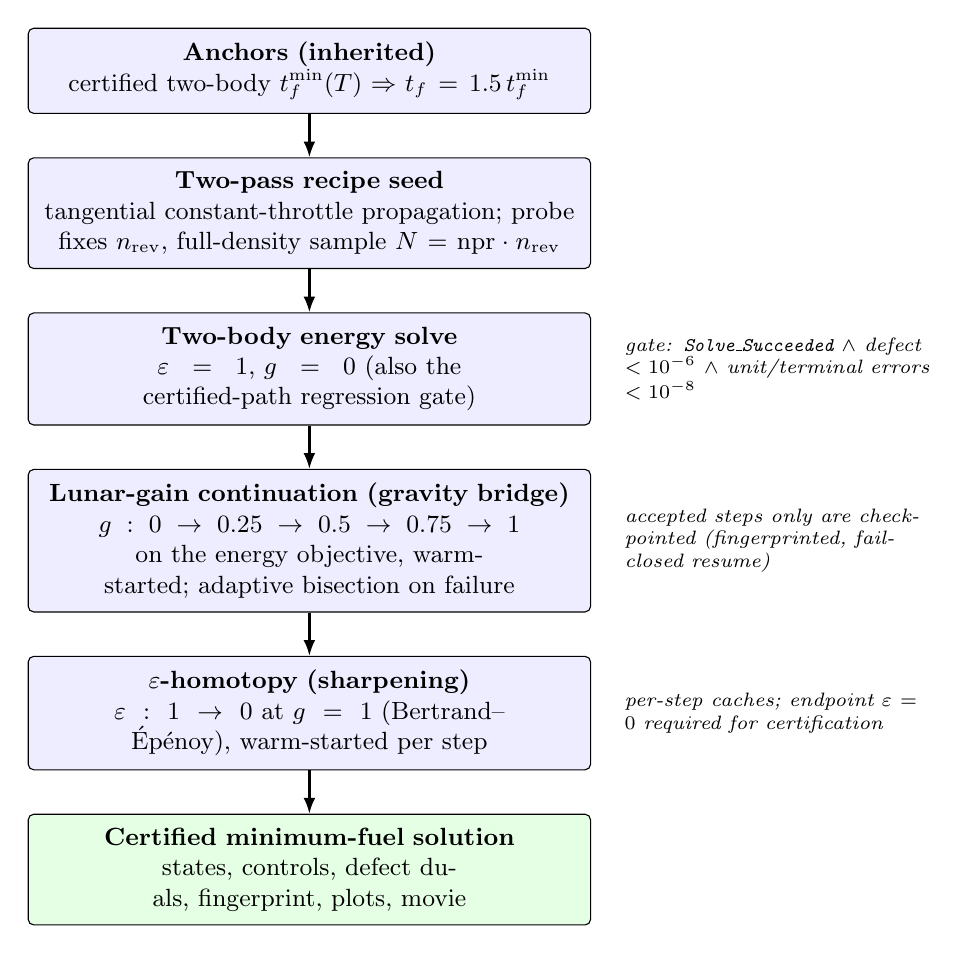
\begin{tikzpicture}[
  node distance=5.5mm,
  box/.style={rectangle, rounded corners=2pt, draw, fill=blue!7,
              text width=0.56\textwidth, align=center, inner sep=5pt, font=\small},
  gate/.style={font=\scriptsize\itshape, text width=0.32\textwidth, align=left},
  arr/.style={-{Latex[length=2mm]}, thick}]
\node[box] (anchor) {\textbf{Anchors (inherited)}\\
  certified two-body $t_f^{\min}(T)$ $\Rightarrow$ $t_f = 1.5\,t_f^{\min}$};
\node[box, below=of anchor] (seed) {\textbf{Two-pass recipe seed}\\
  tangential constant-throttle propagation; probe fixes $n_{\mathrm{rev}}$,
  full-density sample $N = \mathrm{npr}\cdot n_{\mathrm{rev}}$};
\node[box, below=of seed] (e2b) {\textbf{Two-body energy solve}\\
  $\varepsilon = 1$, $g = 0$ (also the certified-path regression gate)};
\node[box, below=of e2b] (mu) {\textbf{Lunar-gain continuation (gravity bridge)}\\
  $g: 0 \to 0.25 \to 0.5 \to 0.75 \to 1$ on the energy objective,
  warm-started; adaptive bisection on failure};
\node[box, below=of mu] (eps) {\textbf{$\varepsilon$-homotopy (sharpening)}\\
  $\varepsilon: 1 \to 0$ at $g = 1$ (Bertrand--\'Ep\'enoy), warm-started
  per step};
\node[box, below=of eps, fill=green!10] (out) {\textbf{Certified minimum-fuel solution}\\
  states, controls, defect duals, fingerprint, plots, movie};
\draw[arr] (anchor) -- (seed);
\draw[arr] (seed) -- (e2b);
\draw[arr] (e2b) -- (mu);
\draw[arr] (mu) -- (eps);
\draw[arr] (eps) -- (out);
\node[gate, right=3mm of e2b.east] {gate: \texttt{Solve\_Succeeded} $\wedge$
  defect $<10^{-6}$ $\wedge$ unit/terminal errors $<10^{-8}$};
\node[gate, right=3mm of mu.east] {accepted steps only are checkpointed
  (fingerprinted, fail-closed resume)};
\node[gate, right=3mm of eps.east] {per-step caches; endpoint
  $\varepsilon = 0$ required for certification};
\end{tikzpicture}
\caption{The Phase-1 solution pipeline. Every arrow is gated; every accepted
step is checkpointed under a configuration fingerprint, so any stage can
resume without recomputation and no stale configuration can silently
warm-start another.}
\label{fig:pipeline}
\end{figure}

\subsection{What we drew from Bonnard--Caillau--Picot}
\label{sec:frompaper}

Four specific things were taken from \cite{BCP2010}:
\begin{itemize}
\item \textbf{The lunar-gain continuation, in the spirit of mass-ratio
  continuation.} Their \S 4.4 computes Earth--Moon transfers by
  continuation in the mass ratio from the Kepler problem, traced to
  Poincar\'e. Our gravity bridge follows that lineage \emph{in spirit}
  rather than literally: the gain $g$ scales only the lunar force in
  Eq.~\eqref{eq:thirdbody}'s contribution to \eqref{eq:gauss}, while the
  lunar mean motion $n_M$ keeps its full-mass CR3BP value throughout, so
  intermediate steps $g \in (0,1)$ trace a homotopy path, not a physical
  CR3BP solution at a reduced mass ratio --- only the $g = 1$ endpoint is
  exact. Their Proposition~2.3 supplies convergence theory relevant to
  this kind of bridge: conjugate-point clearance is a \emph{sufficient}
  nondegeneracy condition for a smooth continuation branch, not an
  if-and-only-if characterization in this generality (regularity of the
  shooting map and endpoint-rank conditions matter too).
\item \textbf{The benign-landscape rationale for bridging on energy.}
  Their Theorem~3.5 proves the \emph{averaged} Kepler energy problem is a
  Riemannian geodesic flow with \emph{empty conjugate and cut loci} in the
  elliptic domain $e \in [0,1)$. That is a theorem about the
  reduced/averaged Kepler problem, not about our unaveraged,
  three-dimensional, time-dependent MEE problem with free $\Delta L$ and
  collocation; we read it as a strong analogy for why energy-first
  continuation is empirically benign here, not a theorem that certifies
  our landscape. It is nonetheless the best theoretical account on hand
  for why every campaign in this repository has found the energy problem
  the reliable continuation backbone, and the reason the Moon is dialed in
  at $\varepsilon = 1$ rather than on the bang-bang fuel problem.
\item \textbf{Conjugate-point certification (adopted as follow-up).} They
  verify local optimality, in their averaged-energy setting and its own
  regularity hypotheses, by integrating the Jacobi (variational) equation
  and checking the first conjugate time exceeds $t_f$. We attribute this
  as the method used in their setting, not a standalone universal
  certificate. Our indirect-side verification is currently first-order
  only; the Jacobi-field check is the recorded upgrade path
  (\S\ref{sec:secondorder}).
\item \textbf{The $\sigma$-bound rev-count law.} Their
  Propositions~3.4/3.7 bound the control sup-norm by an explicit function
  of the geometry over the cumulated longitude, under their stated
  hypotheses. We treat this as a \emph{prospective comparison} --- to be
  checked against those propositions' exact variables and hypotheses once
  the deep-rung ladder results are in hand, not an inherited law for this
  throttle-limited, fixed-time, free-winding formulation --- the rigorous
  cousin of the campaign's empirical
  $T \cdot t_f^{\min} \approx \mathrm{const}$ law.
\end{itemize}
What we did \emph{not} adopt: their averaging-based analytic initialization
(our discrete two-body solutions are stronger seeds), and their
rotating-frame Cartesian formulation --- correct for their Moon-bound
targets, but our GEO target is Earth-bound throughout, which is exactly the
regime where the MEE/perturbation formulation keeps its free-$\Delta L$
advantage.

\subsection{The two continuations in detail}

The three-body minimum-fuel solution is reached by two continuations run in
sequence, each warm-started and gated:

\paragraph{1. Lunar-gain continuation (gravity bridge).}\label{sec:mubridge}
Starting from the certified two-body \emph{energy} solution
($\varepsilon = 1$), the lunar gain is walked $g: 0 \to 1$
(schedule $0.25, 0.5, 0.75, 1.0$, with adaptive bisection on failure). The
gain $g$ scales only the lunar \emph{force} contribution to
\eqref{eq:gauss}; the lunar mean motion $n_M$ retains its full-mass CR3BP
value throughout, so intermediate steps $g \in (0,1)$ trace a homotopy
path rather than a physical CR3BP solution at reduced mass ratio --- only
the $g = 1$ endpoint is exact. This is done in the spirit of the classical
continuation in the mass ratio traced to Poincar\'e and developed for
low-thrust transfers by Bonnard--Caillau--Picot \cite{BCP2010}, whose
convergence theory ties smoothness of that (literal mass-ratio)
continuation branch to conjugate-point clearance as a sufficient
condition. The continuation is run on the energy objective deliberately:
BCP's Theorem~3.5 shows the \emph{averaged} energy problem is a Riemannian
geodesic flow free of conjugate and cut points in the elliptic domain
\cite{BCP2010} --- a strong analogy, not a proof, for our unaveraged
setting, but the best account on hand for why the energy landscape is
benign here too.

\paragraph{2. $\varepsilon$-homotopy (sharpening) at full Moon.}\label{sec:sharpen}
With $g = 1$ frozen, the standard energy$\to$fuel homotopy
$\varepsilon: 1 \to 0$ is run with the perturbation active, reusing the
two-body campaign's homotopy machinery unchanged. The bang-bang structure
is thus resolved exactly once, at the final physics.

Both stages checkpoint only accepted steps under a dedicated tag namespace
with configuration fingerprints (thrust, mass, $I_{sp}$, $t_f$, $\mu_M$,
$D_{EM}$, $n_M$, $\varphi_0$, $g$), so two-body and three-body caches can
never silently cross-seed.

\section{A priori null model}

Before any solve, the expected size of the lunar effect is scaled by the
tidal acceleration at GEO radius,
$a_{\text{tide}} \approx 2\mu_M r / D_{EM}^3 \approx
\SI{7.3e-6}{\meter\per\second\squared}$, compared with the thrust
authority $T/m_0$:

\begin{center}
\begin{tabular}{cccc}
\toprule
rung & $T/m_0$ [\si{\meter\per\second\squared}] & tide/authority & $t_f$ [lunar months]\\
\midrule
10\,N  & $6.7\times 10^{-3}$ & $0.109\%$ & $0.19$\\
1\,N   & $6.7\times 10^{-4}$ & $1.09\%$  & $\sim 2$\\
0.1\,N & $6.7\times 10^{-5}$ & $10.9\%$  & $\sim 19$\\
\bottomrule
\end{tabular}
\end{center}

\noindent
At 10\,N the Moon is a $\sim 0.1\%$ actor over a fifth of a lunar month:
this is an order-of-magnitude scaling, not a rigorous bound, and it
suggests a sub-$0.1$\,kg mass shift whose sign depends on geometry. The
deep rungs are where the Moon becomes a $\sim 10\%$ actor
acting over many lunar months --- the physically interesting regime, and
the recorded next step.

\section{Results at the 10 N rung}

\paragraph{Bridge (energy objective).}
Gate 1 (perturbation absent; certified-path regression):
\texttt{Solve\_Succeeded}, defect $4.6\times 10^{-15}$, terminal error
$\sim 10^{-36}$. Gate 2 ($g = 0$ with the perturbation wired in): solution
drift $8.0\times 10^{-9}$ relative to gate 1 --- the hook itself introduces
no physics. The gain walk then converged on the \emph{first attempt at
every step}, with defects $4$--$6\times 10^{-15}$ and energy-stage final
mass moving from $1359.68$ to $1359.72$\,kg across the walk --- a
$+40$\,g effect at the energy stage, consistent with the null model.

\paragraph{Certified minimum-fuel result.}
The $\varepsilon$-homotopy reached $\varepsilon = 0$ with all
certification metrics green (defect $4.2\times 10^{-15}$, unit-norm
violation $<10^{-8}$, terminal error $<10^{-8}$, no unintended active
state/control bounds beyond the expected throttle bounds
$\delta \in \{0,1\}$):
\begin{center}
\begin{tabular}{lcccc}
\toprule
 & $m_f$ [kg] & $\Delta m_f$ & switches$^{\ast}$ & $t_f$\\
\midrule
two-body (certified)   & $1377.1000$ & ---        & 19 & $5.290$\,d\\
three-body (this work) & $1377.1545$ & $+0.0545$\,kg ($+0.004\%$) & 19 & $5.290$\,d\\
\bottomrule
\end{tabular}
\end{center}
{\footnotesize $^{\ast}$Nodal counts; switch counts are mesh-band
quantities, not exact integers (campaign mesh-convergence protocol).}

\medskip
At the baseline lunar phase the Moon \emph{helps}: the transfer finishes
$54.5$\,g heavier. The effect sits squarely inside the null-model band,
and the bang-bang structure is unchanged at this rung. Whether the sign of
$\Delta m_f$ is generic or specific to $\varphi_0 = 0$ is an open,
recorded question --- at 10\,N the transfer spans only a fifth of a lunar
month, so the Moon is nearly static during the transfer and the effect
plausibly reverses with phase.

\section{Certification basis and limitations}
\label{sec:certification}

The three-body result is certified on solver metrics: full IPOPT
convergence (\texttt{Solve\_Succeeded}, never
\texttt{Solved\_To\_Acceptable\_Level}), post-hoc numerically re-checked
collocation defects at $10^{-15}$, terminal and unit-norm errors below
$10^{-8}$, homotopy endpoint $\varepsilon = 0$ reached, and no unintended
active state/control bounds beyond the expected throttle bounds. This is a
deliberately weaker bar than the two-body campaign's, which additionally
verifies Pontryagin consistency through a primer-vector reconstruction. A
CR3BP-aware version of that verifier now exists
(\texttt{mee\_primer\_switch.m}, commit \texttt{4353387}): it subtracts
the zero-throttle ballistic/lunar bracket from the primer extraction and
its switching-function term before comparing against the solver's own
switches, and reduces identically to the pre-existing two-body formulas
when the perturbation is absent. Run against the certified 10\,N and 5\,N
CR3BP fuel solutions, the primer/switch gate initially \emph{failed}
($32.4^\circ$/$78.4\%$ at 10\,N; $26.7^\circ$/$76.6\%$ at 5\,N), while an
A/B check isolating the lunar-specific coupling term (the
$A_0/\dot L_0$ diagnostic, confirmed $\sim 10^{-5}$) showed removing it
moved those numbers by less than $0.1^\circ$ --- establishing that the
dominant cause was the same pre-existing, eccentricity-correlated raw-dual
(KKT-multiplier) anomaly that failed the pure two-body certified solutions
identically, and not a lunar-specific defect.

That anomaly has since been resolved, and the diagnosis above was correct:
it was not physics at all. The optimizer's convenience dual accessor returns
multipliers in the modelling layer's \emph{canonicalized} constraint
orientation rather than the orientation of the constraint row they pair with
in the stationarity condition $\nabla f + A^{\!\top}\lambda = 0$. Because the
collocation defect canonicalizes row by row, the stored duals carried
entry-wise sign corruption --- magnitudes exact, roughly half the signs
inverted --- which is precisely the signature of a structured, physics-like
rotation. Sourcing the defect duals instead from the raw low-level multiplier
vector, indexed by the defect group's own constraint-row range, is correct by
construction. Two independent checks confirm it: assembling the full
Lagrangian gradient from the raw multipliers gives
$\lVert\nabla_x\mathcal{L}\rVert_\infty = 1.5\times10^{-14}$ with the
tangential control-stationarity residual on burn arcs at $8\times10^{-17}$;
and the rebuilt primer takes the gate to $0.000^\circ$ with $100.00\%$
switching-sign agreement on the CR3BP 10\,N row (and on every two-body rung
from 10\,N to 0.2\,N), with switch-alignment error dropping from
$2.1\times10^{1}$ to $1.5\times10^{-1}$. The four NLP metrics above remain
the primal certification; the first-order Pontryagin gate is now an
\emph{independent} check that these solutions also pass. A conjugate-point
(Jacobi-field) second-order check in the style of \cite{BCP2010} remains a
further, separate follow-up (\S\ref{sec:secondorder}).

Further recorded limitations: the Moon-in-reference-plane idealization
(true CR3BP geometry; real obliquity unmodeled); the four-point lunar-phase
sweep run only at the $10$\,N rung so far (\S\ref{sec:phase}), with no
phase sweep yet at any deep rung; and, now that the full thrust ladder
$10 \to 0.1$\,N has been run (\S\ref{sec:ladder}), what remains open is
\emph{not} whether the deep rungs solve, but (i) a deep-rung $\varphi_0$
sweep to test the phase-averaging interpretation of \S\ref{sec:ladder}
against the observed fixed-phase decline, and (ii) stronger optimality
evidence beyond the first-order certificate (\S\ref{sec:minimality}). The
adaptive-bisection path of the gravity bridge was never exercised at
10\,N (all steps converged first-try) and is untested until a deeper rung
stresses it.

\section{Lunar-phase dependence of the Moon effect}
\label{sec:phase}

With the pipeline validated, the lunar phase at departure $\varphi_0$ ---
deliberately a first-class, fingerprinted parameter (D6) --- was swept at
the 10\,N rung: four solves at $\varphi_0 = 0, \pi/2, \pi, 3\pi/2$,
everything else held fixed, each compared against the \emph{same-chain}
two-body control ($g=0$ through the identical pipeline; $m_f^{2b} =
1377.1025$\,kg). The same-chain baseline matters: certified results from
different pipelines scatter across local basins by up to tens of kilograms,
two orders of magnitude above the lunar signal, so only a baseline sharing
the seed, mesh, and continuation path isolates the Moon.

\begin{center}
\begin{tabular}{cccc}
\toprule
$\varphi_0$ & $m_f$ [kg] & $\Delta m_f$ [g] & Moon\ldots\\
\midrule
$0$      & $1377.1545$ & $+52.0$ & helps\\
$\pi/2$  & $1377.0462$ & $-56.3$ & hurts\\
$\pi$    & $1377.1714$ & $+68.9$ & helps\\
$3\pi/2$ & $1377.0497$ & $-52.8$ & hurts\\
\bottomrule
\end{tabular}
\end{center}

\begin{figure}[htb]
\centering
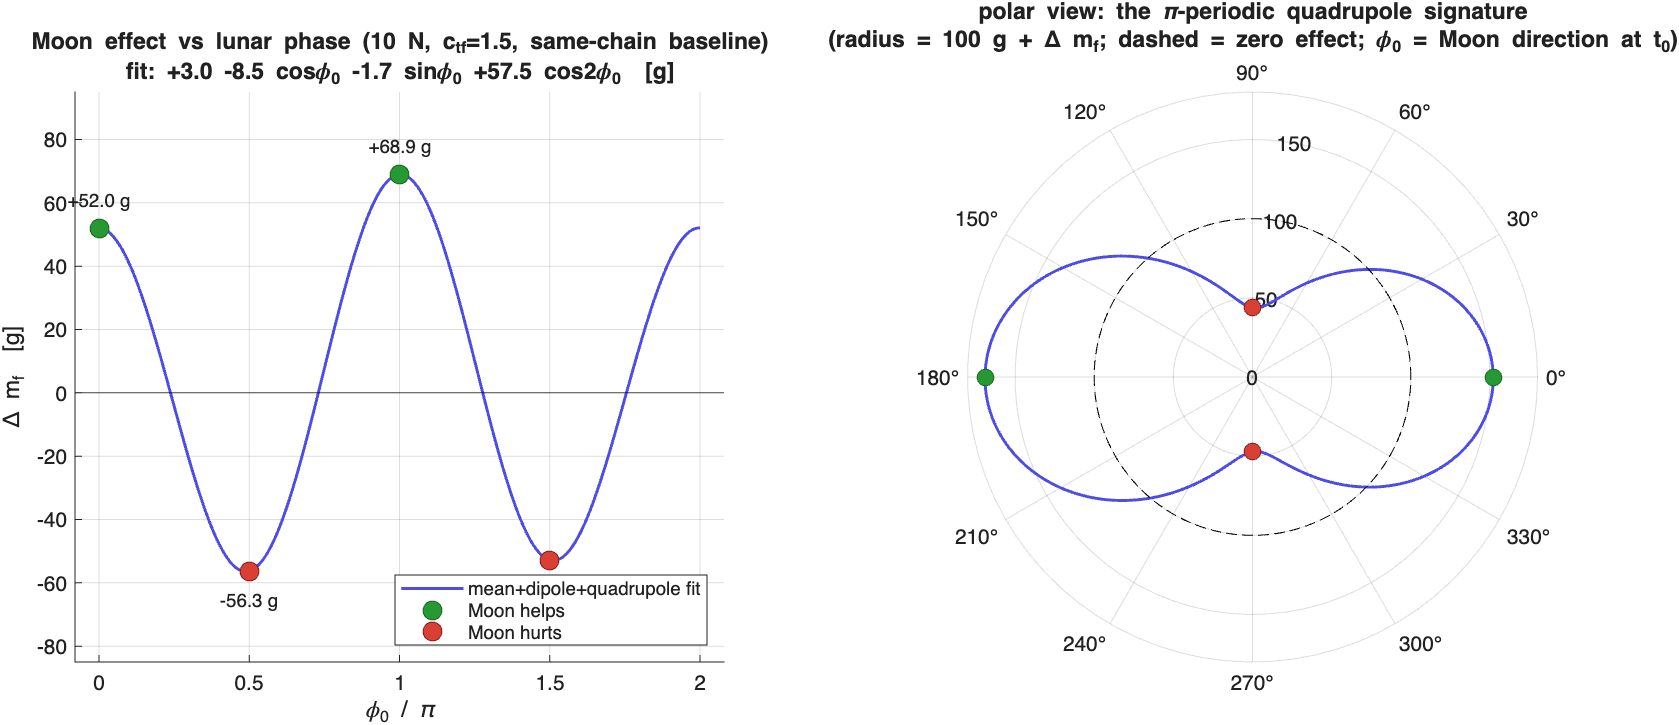
\includegraphics[width=\textwidth]{figs/phi_sweep_dmf.png}
\caption{Moon effect versus lunar phase at 10\,N ($c_{tf}=1.5$, same-chain
baseline). Left: $\Delta m_f(\varphi_0)$ data with the
mean{+}dipole{+}quadrupole fit; right: polar view of the same fit (radius
offset by 100\,g), making the $\pi$-periodic quadrupole lobes along the
$\varphi_0 = 0$--$\pi$ line --- the departure orbit's perigee--apogee line
--- visible at a glance.}
\label{fig:phisweep}
\end{figure}

\paragraph{The signature is a tidal quadrupole.}
The effect \emph{flips sign} with phase and is $\pi$-periodic to leading
order. The four quarter-phase samples fix a mean+dipole+quadrupole fit:
\[
\Delta m_f(\varphi_0) \;\approx\;
\underbrace{+3.0}_{\text{mean}}
\;\underbrace{-\,8.5\cos\varphi_0 - 1.75\sin\varphi_0}_{\text{dipole}}
\;\underbrace{+\,57.5\cos 2\varphi_0}_{\text{quadrupole}}
\quad[\mathrm{g}].
\]
Four cardinal samples at $\varphi_0 = 0, \pi/2, \pi, 3\pi/2$ cannot identify
a $\sin 2\varphi_0$ quadrupole component: that harmonic vanishes identically
at all four sample points, so the displayed fit sets its coefficient to
zero \emph{by construction}, not because the data rule it out --- a finer
$\varphi_0$ grid (already the recorded follow-up below) is required to
measure it. Quadrupole dominance is what the physics prescribes \emph{at
leading order}: the tidal field --- the difference between the direct
lunar attraction and the indirect (Earth-acceleration) term of
\eqref{eq:thirdbody} --- derives at leading order from a potential
proportional to $P_2(\cos\psi)$, which is invariant under Moon\,$\to$\,$-$Moon
reflection. The exact direct-plus-indirect field is \emph{not} itself even
under that reflection at finite lunar distance; finite-distance odd terms
(octupole and higher) are expected on top of the leading $P_2$ symmetry ---
consistent with the nonzero cosine-dipole term observed above, which such
odd terms would produce. At this rung the transfer spans only
$0.19$ lunar months (the Moon sweeps $\sim 70^\circ$ during the transfer),
so departure phase largely fixes the tidal geometry: the Moon along the
perigee--apogee line (either end) aids the transfer; the Moon broadside
hurts it. The smaller dipole term is the finite-distance correction the
pure tide discards --- its sign (stronger benefit at $\varphi_0 = \pi$,
Moon on the apogee side, where the trajectory's slow apogee arcs sit
closest to the Moon) is physically sensible, though with four samples we
do not press the interpretation further.

\paragraph{Operational reading.}
Peak-to-peak the phase choice is worth $\approx 125$\,g at 10\,N ---
propellant obtained purely by choosing the departure epoch within the lunar
month, at zero cost \emph{within this fixed-model optimization} (the NLP
objective, constraints, and time budget are unchanged across $\varphi_0$);
departure-epoch changes are not necessarily free at the mission level ---
launch-window, ground-station, or eclipse constraints can attach a real
cost to shifting epoch that this model does not represent. Whether this
scales at lower
thrust is a sharper question than it appears: as $t_f$ stretches past a
lunar month (0.5\,N and below), the Moon phase-averages over the transfer
and the quadrupole amplitude should collapse --- a concrete, testable
prediction for the deep rungs.

\paragraph{Control-law sensitivity: why identical-looking solutions carry
different verdicts.}
The four solutions are independent optimizations --- nothing constrains
their control laws to agree --- and they do differ, but by strikingly
little. All four share the same 19-switch bang-bang structure; measured
against the $\varphi_0 = 0$ reference, switch crossing times shift by at
most $1.3$ minutes on the $5.3$-day transfer (mean $\lesssim 0.3$ min), no
node anywhere flips between burn and coast, and the largest nodal throttle
difference is $0.04$. Notably, the $\varphi_0 = \pi$ law nearly coincides
with $\varphi_0 = 0$ (maximum shift $0.2$ min) while the broadside phases
shift most --- the quadrupole symmetry expressing itself at the level of
the control law.

The smallness is not an accident but a two-part consequence of optimality.
First, the lunar term is $\sim 0.1\%$ of control authority at this rung and
the switching function's zeros are regular (non-grazing), so an $O(\epsilon)$
perturbation of the dynamics moves each zero by $O(\epsilon)$ --- minutes ---
without creating or destroying switches. Second, and more fundamentally, by
the envelope argument the re-optimized control contributes to the objective
only at \emph{second} order: to first order the entire mass effect is
already captured by the perturbation evaluated along the \emph{unperturbed}
extremal, $\Delta m_f \approx \int_0^{t_f} \lambda^{\!\top}\,
\delta\!f\,\mathrm{d}t$, with the minutes-scale control adjustments adding
only an $O(\epsilon^2)$ correction. This is why the four panels of the
accompanying comparison movie are visually indistinguishable while their
outcomes differ by over $100$\,g peak-to-peak: the physics lives in the
perturbing field acting along an essentially common trajectory, not in the
(nearly unchanged) steering. It also underwrites the experimental design:
the four chains share literally identical Moon-free stages (seed and
two-body energy solve), so every reported difference is purely
lunar-phase-driven. The measurement script is
\texttt{direct/phase\_control\_sensitivity.m}.

\paragraph{Caveats.}
Four samples identify harmonics only through second order; components of
order three and higher alias into the printed coefficients (a finer
$\varphi_0$ grid is the recorded follow-up). The sweep is at a single rung
and a single basin family, and each point carries the same first-order
certificate as the rest of the campaign (\S\ref{sec:certification}).

\section{The thrust ladder: results, lessons, and conclusions}
\label{sec:ladder}

The campaign's second sweep held $\varphi_0 = 0$ and walked the full HMG
thrust ladder, $10 \to 0.1$\,N, each rung a complete front-door chain
(recipe seed $\to$ two-body energy $\to$ lunar-gain continuation $\to$
$\varepsilon$-homotopy) paired with its own same-chain $g=0$ control:

\begin{center}
\begin{tabular}{ccccc}
\toprule
$T$ [N] & $t_f$ [lunar mo] & switches & $\Delta m_f$ [g] & defect\\
\midrule
$10$  & $0.19$  & $19$   & $+52.0$ & $4\times10^{-15}$\\
$5$   & $0.39$  & $36$   & $+48.8$ & $1\times10^{-14}$\\
$2.5$ & $0.78$  & $70$   & $+49.7$ & $3\times10^{-14}$\\
$1$   & $1.95$  & $178$  & $+49.3$ & $5\times10^{-14}$\\
$0.5$ & $3.89$  & $357$  & $+45.9$ & $1\times10^{-13}$\\
$0.2$ & $9.72$  & $890$  & $+36.8$ & $2\times10^{-13}$\\
$0.1$ & $19.45$ & $1724$ & $+31.3$ & $5\times10^{-13}$\\
\bottomrule
\end{tabular}
\end{center}

\begin{figure}[htb]
\centering
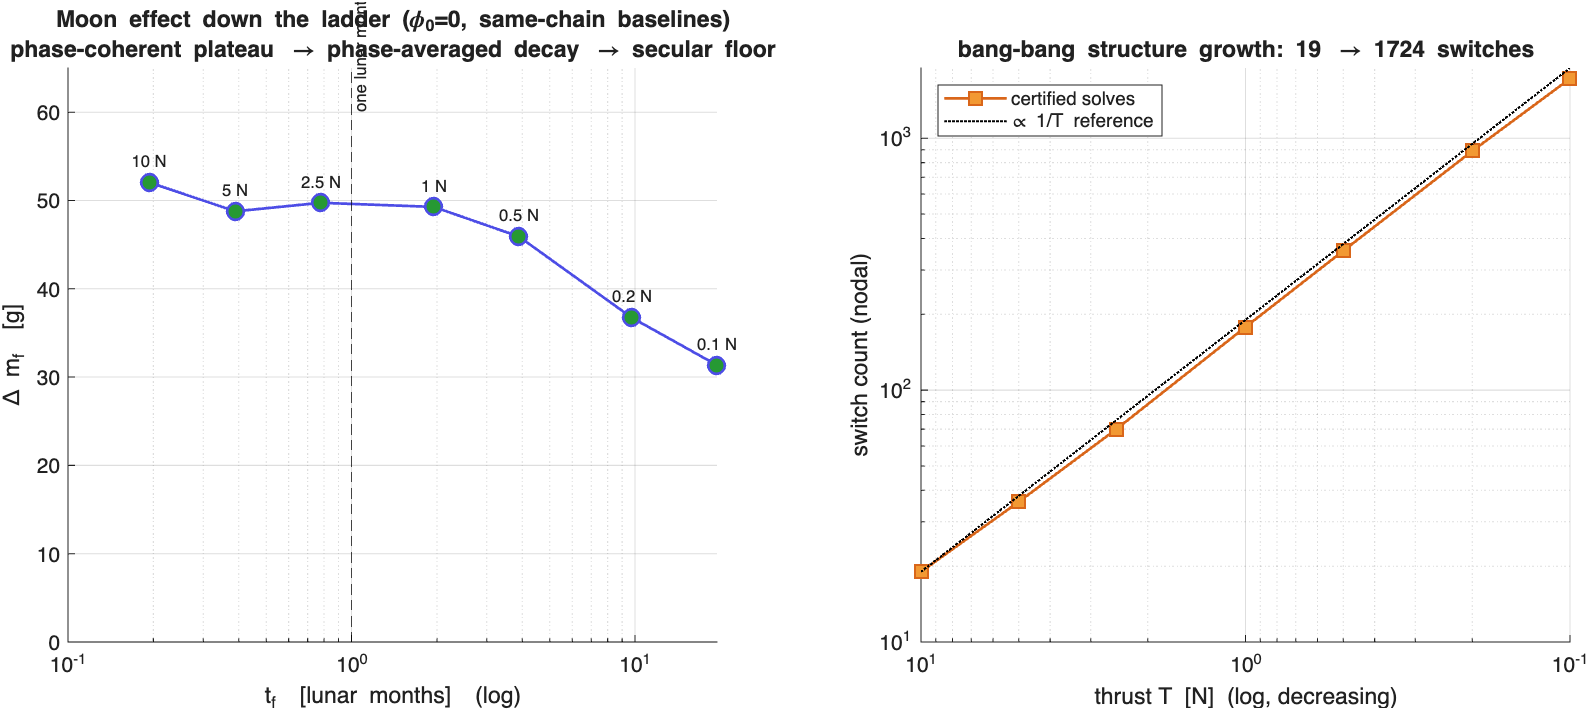
\includegraphics[width=\textwidth]{figs/ladder_dmf.png}
\caption{Left: the Moon effect down the ladder against transfer time in
lunar months (same-chain baselines throughout) --- a phase-coherent plateau
near $50$\,g while $t_f \lesssim 2$ lunar months, then a gentle
phase-averaged decay toward a nonzero secular floor ($\approx 30$\,g at
$19$ months). Right: bang-bang structure growth, $19 \to 1724$ switches,
tracking a $1/T$ reference across two thrust decades (switch counts are
nodal, mesh-band quantities).}
\label{fig:ladder}
\end{figure}

\subsection{Two regimes: what is observed, what is hypothesized}

Read together with \S\ref{sec:phase}, the ladder's fixed-phase
($\varphi_0 = 0$) data support the following observations directly: the
effect plateaus near $+50$\,g through roughly two to four lunar months of
transfer time --- the $1.95$-month point is still $+49.3$\,g, so the
plateau persists at least that far --- and then declines to $+31.3$\,g at
$19.45$ months. The decline therefore sets in somewhere between the
$3.89$-month ($+45.9$\,g) and $9.72$-month ($+36.8$\,g) points, \emph{not}
at the one-lunar-month mark a naive reading of ``the plateau lasts about a
month'' would suggest.

The natural INTERPRETATION, read against \S\ref{sec:phase}'s quadrupole
decomposition, is that while the transfer is short against the lunar month
the $\varphi_0$-dependent quadrupole dominates and the plateau value is
simply the $\varphi_0 = 0$ slice of that curve; as $t_f$ stretches past a
lunar month the Moon sweeps many cycles during the transfer, the
quadrupole contribution averages down, and what survives approaches a
phase-independent secular benefit. This is an interpretation, not a
second measurement: it remains untested until a $\varphi_0$ sweep is run
at a deep rung (the testable corollary below), since the fixed-phase
ladder by itself cannot distinguish ``quadrupole averaging to a floor''
from any other mechanism producing the same $\varphi_0 = 0$ curve.

The interpretation does \emph{not} let the $10$\,N phase-mean stand in for
the deep-rung floor. \S\ref{sec:phase}'s harmonic fit gives a phase-mean of
only $+3.0$\,g at $10$\,N, far below the observed $+31.3$\,g at $0.1$\,N;
if the averaging picture is right, the phase-independent (secular)
component of the Moon effect is \emph{not} constant down the ladder --- it
must itself grow with transfer time, from a few grams' worth of secular
signal at $10$\,N to something approaching the observed $31.3$\,g by
$0.1$\,N. The deep-rung phase-mean is therefore a prediction to be
checked against the sweep, not a quantity already implied by the $10$\,N
decomposition.

Two further statements follow from this interpretation and are flagged as
PREDICTIONS, not measurements: that departure-epoch choice is worth
approximately nothing at the slow end (because the quadrupole is
predicted to have averaged away), and that the slow end keeps a secular
benefit near the observed $31.3$\,g regardless of epoch (because that
secular component is predicted to be phase-independent). Only the
$31.3$\,g figure itself, at $\varphi_0 = 0$, is an observed fixed-phase
value; peak-to-peak epoch sensitivity is $\sim 125$\,g at the fast ($10$\,N)
end, also observed. A directly testable corollary (recorded, not yet run):
a $\varphi_0$ sweep at $0.2$ or $0.1$\,N should show the quadrupole
amplitude collapsed and its phase-mean approaching the observed
fixed-phase value of $\approx 31$\,g.

\subsection{Lessons learned}

\begin{enumerate}
\item \textbf{Formulation choice decides factorization viability.} Every
  rung at or below $2.5$\,N ($N \gtrsim 700$ nodes) segfaulted inside the
  bundled MUMPS at one reproducible instruction --- the in-place workspace
  compression during numerical factorization. Neither single-threading
  (which traded the crash for a quasi-hang) nor enlarged MUMPS workspace
  cured it. The cure was already on the shelf: the solver's lifted
  $\Delta L$ option, added by an earlier external review precisely because
  the scalar span's dense column produces a bordered (``arrowhead'') KKT
  hostile to sparse factorization at large $N$. Lifting is numerically
  identical and block-banded; with it, the entire ladder ran without a
  single factorization failure.
\item \textbf{Iteration budget is decisive --- again.} The lifted cold
  energy solve at $2.5$\,N stalls at $1500$ iterations (defect
  $7\times10^{-6}$, terminal error already tight) and certifies cleanly at
  $4000$; the deepest rungs used $10^4$. The same lesson the two-body
  campaign's deep rungs taught: an under-budgeted solve looks like a wall.
\item \textbf{The predicted deep-rung wall did not exist.} Our prior
  two-body campaign needed dedicated machinery (adaptive-$\varepsilon$
  bisection, staged recovery) at $0.2$/$0.1$\,N; this campaign's front-door
  chain, lifted and properly budgeted, carried both rungs through
  $\varepsilon \to 0$ on the standard schedule. The new results show that
  wall was not intrinsic to sharpening: lifting was necessary to remove the
  factorization failures reported above. But lifting, the larger iteration
  budgets (previous lesson), and this campaign's revised front-door chain
  were all changed at once, so this evidence is \emph{confounded} --- it
  does not by itself isolate lifting's contribution from the budget or
  chain changes. An unlifted, equally-budgeted A/B run on the same chain is
  the clean test and has not been done.
\item \textbf{Same-chain baselines are mandatory at this signal size.}
  Certified results from different pipelines scatter across local basins
  by up to $\sim 22$\,kg --- more than 400 times the $\sim 50$\,g lunar
  signal. Two rungs of this ladder landed in basins $9$--$14$\,kg better
  than the two-body campaign's certified table rows. Every $\Delta m_f$
  reported here is therefore differenced against a $g=0$ control run
  through the identical seed, mesh, and continuation path.
\item \textbf{Fail-loud caches carried their weight.} The fingerprinted,
  fail-closed checkpoint system (built after an earlier review) refused
  stale configurations on at least three occasions during the ladder ---
  including twice against the authors' own scripting mistakes. Every
  refusal was correct.
\item \textbf{Per-rung process isolation.} Running each rung in its own
  interpreter process converted an uncatchable library crash from a
  campaign-killer into a per-rung retry, and made the crash forensics
  (identical faulting instruction across five rungs) possible at all.
\end{enumerate}

\subsection{Conclusions}

For minimum-fuel elliptic$\to$GEO transfers at CR3BP fidelity: lunar
gravity moves the optimal final mass at the $10^{-5}$ level (tens of
grams on $1500$\,kg), with a structure that is now quantitatively mapped
--- a departure-phase quadrupole of amplitude $\approx 57$\,g in the
phase-coherent regime, observed declining from a $\sim 2$--$4$-month
plateau to $+31.3$\,g at $19.45$ months --- consistent with, but not yet
confirming, a phase-independent secular floor, which remains a hypothesis
pending a deep-rung $\varphi_0$ sweep. At this problem's
scale the Moon is thus a refinement, not a design driver; but the
methodology result is broader: the Earth-centered MEE formulation with an
opt-in third-body term, gain continuation on the energy objective, and the
standard $\varepsilon$-homotopy scaled \emph{unchanged} across two decades
of thrust, $19 \to 1724$ switches, and transfer times from five days to
seventeen months --- with the free-$\Delta L$ (lifted) span identified as
the load-bearing formulation choice at scale. The usual caveats stand:
switch counts are nodal mesh-band quantities, certificates are first-order
(\S\ref{sec:certification}), deep-rung defects grow to $5\times10^{-13}$ (seven orders inside
the gate), and all results live in one basin family per rung.

\section{Direct versus indirect methods: a working position}

\emph{This section is deliberately speculative} --- it records campaign
\emph{observations}, not a categorical law, to be revised as evidence
accumulates. The organizing axis we have found most predictive is
\textbf{sensitivity versus combinatorics}: indirect (PMP shooting) methods
have tended to degrade with \emph{arc sensitivity} --- the shooting
Jacobian is a state transition matrix whose norm we have observed to grow
roughly exponentially with revolution count, amplified at each deep
perigee pass, \emph{in the single-shooting formulations tried so far} ---
while direct (collocation) methods degrade with \emph{combinatorial
structure} (bang-bang switch discovery) and mesh resolution. Shooting
sensitivity is problem-, scaling-, and formulation-dependent, and is a
known mitigable failure mode in the wider literature: multiple shooting
and conjugate-point-guarded continuation (as in the exception below) both
reduce it. We have not yet tried multiple shooting on this campaign's deep
rungs; the observation above describes what single shooting has done here,
not a proof that it must.

The resulting division of labor, as observed on this repository's
campaigns to date:
\begin{itemize}
\item \textbf{Minimum time at low thrust (many revolutions): direct.}
  All-burn means no switching structure, so collocation's weakness is
  absent, while the long sensitive arc is single shooting's worst case.
  Every certified min-time anchor in this repository is a direct solve.
\item \textbf{Minimum fuel, structure unknown: direct + homotopy for
  discovery.} The $\varepsilon$-continuation finds the bang-bang structure
  without knowing it a priori. Caveat: switch \emph{counts} from a fixed
  mesh are band quantities, not exact integers.
\item \textbf{Precision and certification once seeded: indirect.} With the
  structure known and costates seeded from a converged direct solution, a
  shooting solve has, in the cases run so far, delivered machine-precision
  switch times and costates at low cost --- its weakness (initialization)
  having been paid by the direct stage. This is not automatic: it requires
  a correct multiplier/costate mapping from the direct solution's KKT
  duals and a conditioning check on the resulting shooting Jacobian before
  the result is trusted; neither is guaranteed by seeding alone. With those
  checks passed, the direct-seeded indirect finish is, in our view, a
  strong marriage.
\item \textbf{The instructive exception} \cite{BCP2010}: indirect shooting
  \emph{does} work at 50--60 revolutions when the objective is the smooth
  energy one, the initializer is an averaged analytic solution, and the
  continuation is conjugate-point-guarded --- i.e., high revolution count
  kills \emph{cold or unguarded single} shooting, and nonsmooth structure
  compounds it, but neither is fatal alone, and standard mitigations
  (multiple shooting, guarded continuation) are available.
\end{itemize}
For this campaign specifically: the Phase-1 pipeline is direct end-to-end;
the indirect counterpart (Phase 2) is planned as a direct-seeded finisher
whose payoff is precision switch times and a second-order certificate
(\S\ref{sec:minimality}), not discovery.

\section{Refinement and stronger optimality evidence}
\label{sec:minimality}

\subsection{Switch-time refinement (PSR): yes, eventually}

Both sibling campaigns carry post-solution refinement (PSR) machinery: the
two-body ladder used PSR rounds at its 0.5\,N rung, and the GTO--tulip
campaign built PMP-steered mesh refinement in which the reconstructed
switching function steers local mesh densification at each switch. The same
step belongs in this campaign's future --- switch times from a uniform
$\sigma$-mesh are only mesh-band accurate, and at deep rungs (hundreds of
switches) the uniform mesh under-resolves switch clusters. The prerequisite
this once gated on --- a lunar-aware switching function --- is now built
(\S\ref{sec:certification}, commit \texttt{4353387}): the primer/switch
reconstruction correctly subtracts the ballistic third-body rate under
lunar gravity. The second prerequisite --- that the reconstruction actually
agree with the solver's own switches --- was for a time the binding one: PSR
consumes the same primer/switching reconstruction, which disagreed by tens
of degrees at both certified CR3BP rungs. That disagreement has since been
traced to the dual-extraction defect described in \S\ref{sec:certification}
(a constraint-orientation mismatch in the optimizer's convenience dual
accessor, not a property of the trajectories) and corrected. With duals taken
from the raw multiplier vector, the reconstruction now reproduces the
solver's switches to a switch-alignment error of $1.5\times10^{-1}$ against a
primer misalignment of $0.000^\circ$. Both prerequisites are therefore met
and PSR is unblocked; it is scheduled work rather than a blocked item, and
remains required before any switch-time claim at the deep rungs, where a
uniform mesh under-resolves switch clusters.

\subsection{Toward genuine local-minimality certificates}
\label{sec:secondorder}

Everything certified so far is \emph{first-order}: IPOPT's KKT conditions,
machine-tight defects, endpoint and structure checks. A converged extremal
satisfying first-order conditions can still be a saddle or a local
maximizer of the induced problem. The plan for genuinely second-order
evidence has three tiers, in order of readiness:
\begin{enumerate}
\item \textbf{NLP-level SOSC (machinery partially built).} The shared
  solver already exposes \texttt{returnModel} --- the live constraint and
  variable registries assembled precisely for KKT/reduced-Hessian work, with
  a design plan (\texttt{PLAN\_sosc.md}) in the two-body campaign. The
  check: project the Lagrangian Hessian onto the null space of the active
  constraints and verify positive definiteness. This certifies the
  \emph{discretized} problem's minimality and is the cheapest tier to
  finish.
\item \textbf{Bang-bang second-order conditions via the induced
  switching-time problem.} For bang-bang arcs the right continuous-time
  frame (Maurer, Osmolovskii) reduces the OCP to a finite-dimensional
  problem in the switch times; positive definiteness of that induced
  Hessian, together with no additional zeros of the switching function, is
  a genuine sufficient condition \emph{under} the accompanying hypotheses
  --- normality of the extremal, regular (strict, transversal) switching
  with no singular arcs, the relevant endpoint constraint qualification,
  and positivity/coercivity of the induced Hessian on the appropriate
  critical cone. Absent those, positive definiteness plus no extra zeros
  certifies only the topology-fixed, finite-dimensional switching-time
  reduction, not the full OCP. Naturally shared with PSR: both live on the
  arc-parameterized representation.
\item \textbf{Indirect-side conjugate-point test.} Integrate the Jacobi
  (variational) equation along the extremal and verify no conjugate time in
  $(0, t_f]$ \cite{BCP2010} --- not, by itself, a generic classical
  certificate: it requires the associated strengthened Legendre condition
  and endpoint regularity hypotheses from BCP's setting, and it certifies
  \emph{weak} local optimality (optimality against nearby extremals of the
  same structure), which is distinct from \emph{strong} local optimality
  and from global minimality. Planned with the Phase-2 indirect solver, and
  dependent on the same CR3BP-aware costate reconstruction as PSR.
\end{enumerate}
Until these land, the honest statement remains: our solutions are
first-order certified extremals whose optimality is corroborated by
basin-reference checks and cross-formulation agreement, not proven minima.

\begin{thebibliography}{9}

\bibitem{HMG2004}
T.~Haberkorn, P.~Martinon, J.~Gergaud,
``Low-thrust minimum-fuel orbital transfer: a homotopic approach,''
\emph{Journal of Guidance, Control, and Dynamics} 27(6), 2004.

\bibitem{CN2001}
J.-B.~Caillau, J.~Noailles,
``Coplanar control of a satellite around the Earth,''
\emph{ESAIM: Control, Optimisation and Calculus of Variations} 6, 2001.

\bibitem{BE2002}
R.~Bertrand, R.~\'Ep\'enoy,
``New smoothing techniques for solving bang-bang optimal control problems,''
\emph{Optimal Control Applications and Methods} 23(4), 2002.

\bibitem{BCP2010}
B.~Bonnard, J.-B.~Caillau, G.~Picot,
``Geometric and numerical techniques in optimal control of two and
three-body problems,''
\emph{Communications in Information and Systems} 10(4), 239--278, 2010.

\bibitem{Betts2010}
J.~T.~Betts,
\emph{Practical Methods for Optimal Control and Estimation Using Nonlinear
Programming}, 2nd ed., SIAM, 2010.

\end{thebibliography}

\end{document}
